\section{Abundance decrement trends}
\label{sec:trends}

Star-forming galaxies have been shown to possess similar metallicity gradients across a range of total stellar masses \citep{sanchez_2014_metgrad, belfiore_2017_manga-metgrad, mingozzi_2020}, with some evidence that gradients steepen with increasing galaxy stellar mass \citep{belfiore_2017_manga-metgrad, poetrodjojo_18, mingozzi_2020}. Figure \ref{fig:logmass-dec01-hifrac} illustrates that despite broadly consistent radial metallicity decrements across a range of galaxy stellar masses, there is also great diversity at fixed mass. Likewise, a wide range of HI mass fractions exist at similar stellar mass. Before exploring the origin of the dispersion in measured decrement at fixed stellar mass, and its relation to HI, we consider how our decrements compare to previous measurements of abundance gradient.

\begin{figure*}
    \centering
    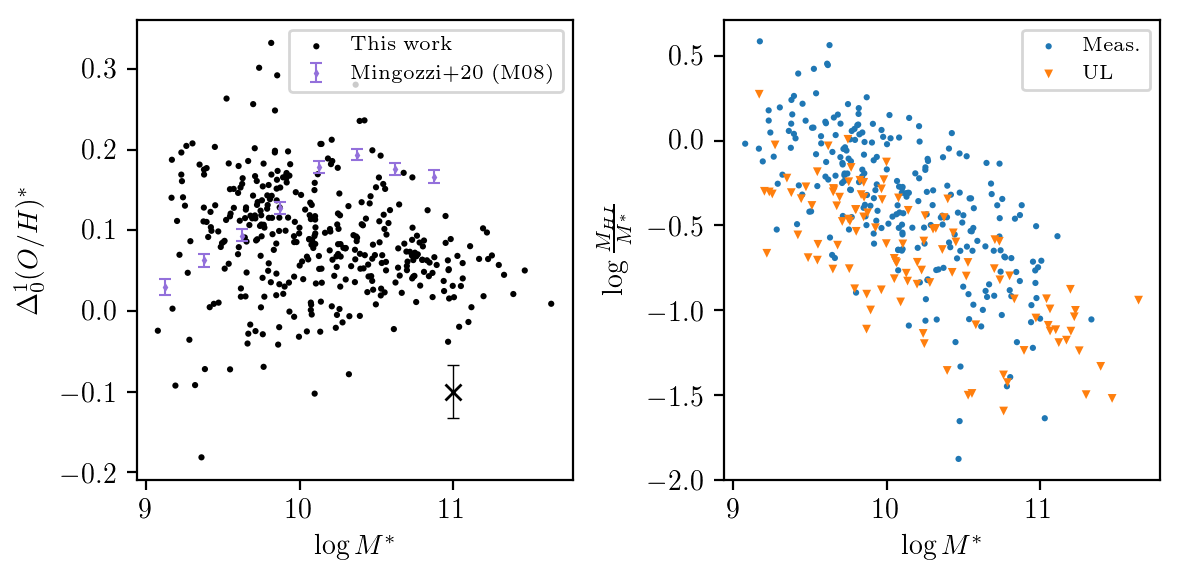
\includegraphics[width=5in]{logmass-dec01-hifrac}
    \caption[The correlations between total galaxy stellar mass, radial abundance decrement, and \hifrac, overlaid with transformed literature values.]{\fixspacing The relationships between total galaxy stellar mass, radial abundance decrement ($\metdec = (12 + \log \frac{O}{H})_{inner} - (12 + \log \frac{O}{H})_{outer})$ between the first two radial bins, and \hifrac. A positive decrement indicates a radially-decreasing gas-phase metallicity profile. In the left-hand panel, stellar mass is shown on the abscissa and \metdec on the ordinate (a representative uncertainty for \metdec is also shown). We also show the mass-dependent radial decrements arising from the median radial gradients calculated in \citet{mingozzi_2020}, assuming a uniform gradient from $0.25-1.5 ~ R_e^t$ (note the radial unit of \emph{total effective radii}). In the right-hand panel, we show the logarithm of the ratio between stellar mass and HI mass (positive detections are blue circles, upper-limits are orange, downward-facing triangles). While there is of course a broad trend of decreasing \hifrac with $M^*$, the scatter about that trend is significant (likely $\gtrsim 0.3 ~ {\rm dex}$, or a factor of several). Similarly, the scatter in \metdec at fixed stellar mass becomes most significant at $\logmstar \lesssim 10.5$.}
    \label{fig:logmass-dec01-hifrac}
\end{figure*}

\subsection{Decrements vs. gradients}
The relationship between a radial decrement and a gradient is intuitive: after adopting endpoints of $0.25 ~ R_e^t$ and $1.75 ~ R_e^t$ (the midpoints of the inner and outer radial intervals), the median measured metallicity gradients obtained in \citet[a recent study using MaNGA data]{mingozzi_2020} can be transformed into decrements, for comparison to this work (Figure \ref{fig:logmass-dec01-hifrac}, light purple points with errorbars). At low stellar mass ($\logmstar < 10$), the median radial gradient from \citet{mingozzi_2020} is well within the range of individual decrements measured in this work. It is crucial to note that the \citet{mingozzi_2020} points represent constraints on the \emph{median radial abundance trend} at fixed mass, rather than the \emph{true distribution of metallicity gradients}\footnote{The \citet{mingozzi_2020} median gradients were found by first aggregating individual galaxies' spaxels into radial bins, and then fitting all galaxies in a stellar mass bin with one linear regression against galactocentric radius}. The transformed gradients of \citep{mingozzi_2020} do differ from this works' results at higher stellar mass ($\logmstar \ge 10$). Some combination of the following effects are likely responsible:
%
\begin{itemize}
    \item \citet{mingozzi_2020} uses a similar, but not identical $R_{23}$ strong-line metallicity calibration defined in \citet[Table 4]{maiolino_nagao_2008}, which relies on ``direct" $T_e$ metallicities at $\met < 8.4$ and photoionization models at higher abundance. \citet{belfiore_2017_manga-metgrad} has shown that changing the strong-line metallicity calibration affects gradients and their trends with mass, so similar differences are expected here.
    \item The gradients of \citet{mingozzi_2020} were found in \emph{total effective radius} ($R_e^t$) coordinates (rather than the \emph{disk effective radius} coordinates used for this work's empirically-measured gradients). This means galaxies with prominent bulges will produce gradients that are too steep. 
    \item \citet{mingozzi_2020} fit the radial gradients only between $0.5-2.0 ~ R_e^t$, excluding nearly the full breadth of the innermost radial annulus adopted in this work, in order to sidestep non-linear radial profiles (in particular, the well-known flattening of the abundance profile inward of $1.0 ~ R_e$).
\end{itemize}
%

\subsection{Radial metallicity trends and HI}

Does HI content exert an influence over \metdec beyond its correlation with stellar mass? Figure \ref{fig:hifrac_dec01_subplotmstar} shows evidence of a positive correlation between HI mass fraction and radial gas-phase metallicity decrement, when galaxies are separated by their total stellar mass into four bins. The bins are set as the 16$^{th}$, 50$^{th}$, and 84$^{th}$ percentiles of the stellar-mass distribution of galaxies with either an H\textsc{i} mass measurement or upper-limit: $10^{9.6}$, $10^{10.1}$, and $10^{10.7}~{\rm M_{\odot}}$. The correlation manifests for galaxies with measured HI masses as well as upper-limits.

Since a steep decrement could emerge from a high central value, rather than a low outer value, a positive correlation between central metallicity and HI mass might feasibly bring about the observed correlation between strong decrement and HI mass fraction. In practice, though, galaxies with the largest HI fractions at fixed stellar mass also have \emph{lower-than-typical gas-phase metallicities} in their inner 0.5 $R_e$. This is consistent with the standard picture of galaxy chemical evolution \citep{tinsley_72, tinsley_73}, and qualitatively similar to other observed relations between gas fraction and oxygen abundance \citep{hughes_2013-gfrac-met}. Thus, we conclude that the correlation is not an emergent result of differing galaxy-to-galaxy abundance zeropoints.

The correlation we observe between a steep radial metallicity profile and a large HI mass is reminiscent of a result noted in a sample of DustPedia galaxies with archival MUSE integral-field spectroscopic observations \citep{devis_2019_dustpedia}. The DustPedia parent sample has a great breadth of photometric measurements (25 bands from UV to submillimeter); but there are only 75 galaxies with integral-field spectroscopic observations (from the MUSE archive), albeit with finer spatial sampling than MaNGA reaches. Radial metallicity trends are measured in \citet{devis_2019_dustpedia} with a linear fit, and are a true gradient over the entire galaxy, though with respect to $r_{25}$ (the radius of the $m_B = 25$ isophote). Though converting between gradients in the units of $r_{25}$ (DustPedia) and the decrements in the units of disk effective radii (this study) is not straightforward, we note with interest that there is some basis for a \metdec-HI correlation in the literature.

\begin{figure*}
    \centering
    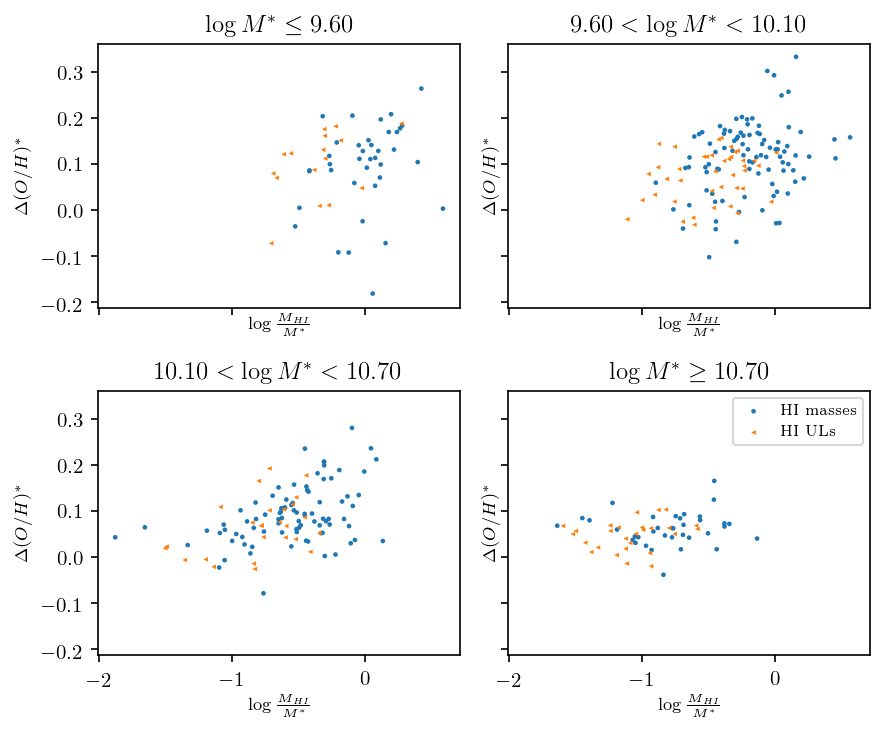
\includegraphics[width=\textwidth]{hifrac_dec01_subplotmstar}
    \caption[The correlation between radial metallicity decrement and \hifrac, separated by total galaxy stellar mass.]{\fixspacing The radial oxygen abundance decrement between $0.0-0.5 ~ R_e$ \& $1.25-1.75 ~ R_e$ (\metdec) is shown on the abscissa, with respect to the HI mass normalized by the stellar mass ($\log M_{HI} / M^*$). Positive HI detections are shown as blue squares, and upper-limits as orange triangles: at fixed total stellar mass, the atomic gas mass upper-limits probe a lower gas-fraction branch of the galaxy population. There is a moderate correlation between HI mass fraction and oxygen abundance decrement strength at fixed galaxy total stellar mass, present most prominently at $M^* < 10^{10.7} {\rm M_{\odot}}$.}
    \label{fig:hifrac_dec01_subplotmstar}
\end{figure*}

Since gas-phase metallicity is a manifestation of a galaxy's (or a region's) chemical evolution, an abnormal metallicity decrement could indicate that an inflow has disturbed the galaxy's abundance profile: such a galaxy might be in an abnormal or non-steady state, with oxygen abundance varying azimuthally as well as radially. We therefore now consider the width of the gas-phase metallicity distribution within the outer radial bin ($1.25-1.75 ~ R_e$), \metdisp, defined as the median absolute deviation distribution of spaxel oxygen abundances within that radial interval. Since \metdisp signifies heterogeneity in chemical enrichment within the outermost radial bin, it is a fair proxy for azimuthal variations in gas-phase metallicity at fixed radius. Figure \ref{fig:madoh1_dec01_subplotmstar} shows the relationship between \metdisp and \metdec in the same four stellar-mass bins used in Figure \ref{fig:hifrac_dec01_subplotmstar}; and Figure \ref{fig:madoh1_hifrac_subplotmstar} shows the relationship between $\log M_{HI} / M^*$ and \metdisp. There is indeed a positive correlation between a strong radial decrement and large metallicity dispersion within a single radial bin; and also between gas-richness \& \metdisp. This implies a close relationship between gas content and non-uniform chemical evolution across a single galaxy.

\begin{figure*}
    \centering
    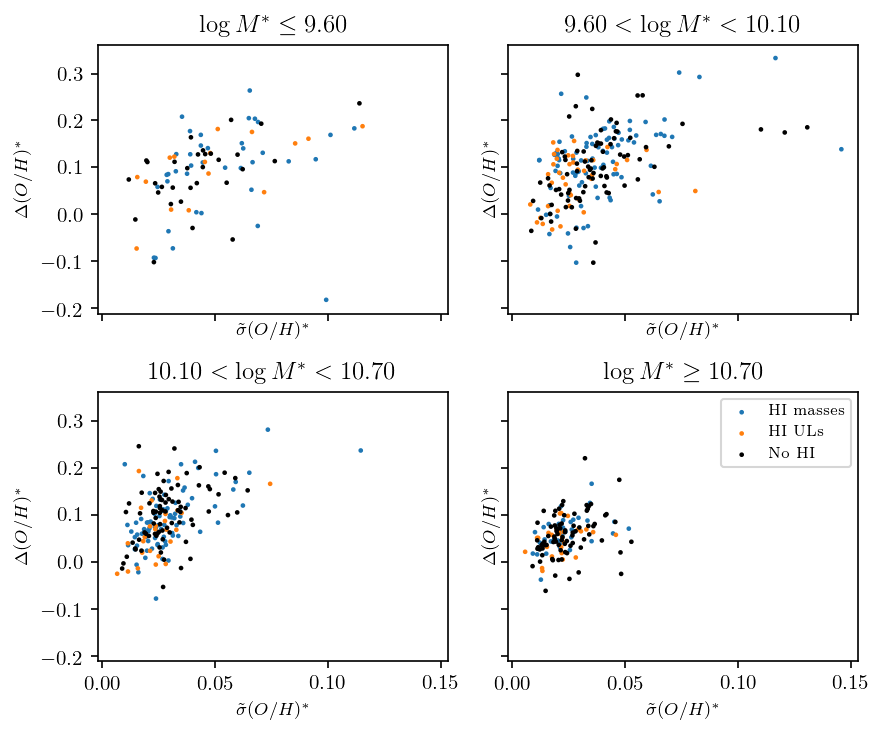
\includegraphics[width=\textwidth]{madoh1_dec01_subplotmstar}
    \caption[As Figure \ref{fig:hifrac_dec01_subplotmstar}, but relating dispersion of gas-phase metallicity at fixed radius with the strength of metallicity decrement.]{\fixspacing As Figure \ref{fig:hifrac_dec01_subplotmstar}, but relating dispersion of gas-phase metallicity at fixed radius (abscissa) with the strength of metallicity decrement (ordinate), when galaxies are separated by their total stellar mass. Within individual stellar-mass bins, there is a visual correlation between \metdisp and \metdec (see Table \ref{tab:dec-corr_mstarsep} for Kendall's $\tau$ correlation coefficients accounting for upper-limits). This is true for galaxies with measured HI masses (blue), HI upper-limits (orange), and with no measured HI at all (black). The correlation is most striking in the three lower-mass bins, and is marginal for $M^* > 10^{10.7} {\rm M_{\odot}}$.}
    \label{fig:madoh1_dec01_subplotmstar}
\end{figure*}

\begin{figure*}
    \centering
    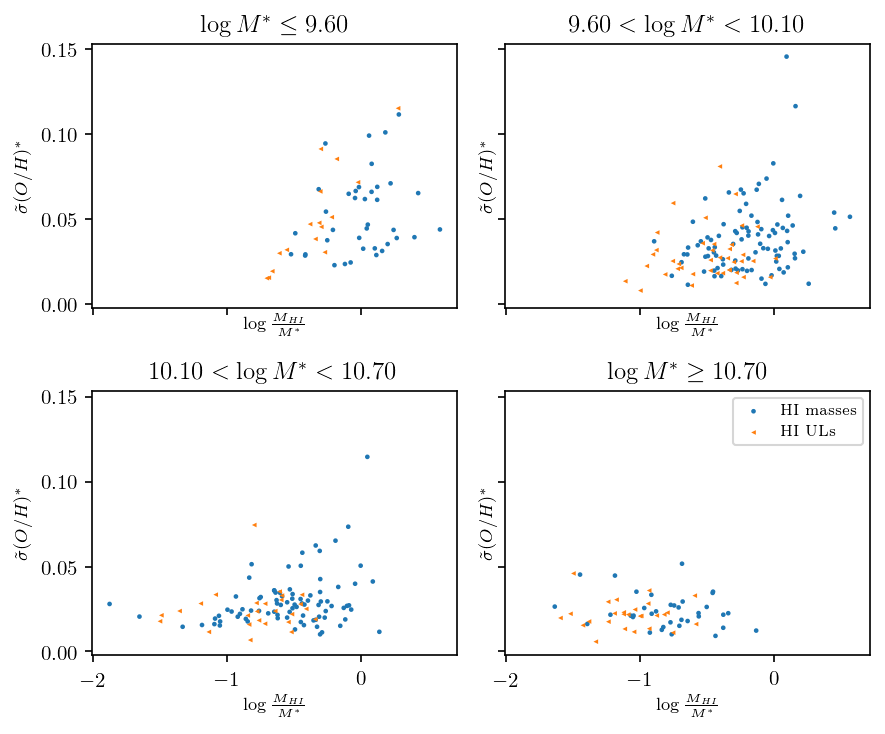
\includegraphics[width=\textwidth]{hifrac_madoh1_subplotmstar}
    \caption[As Figures \ref{fig:hifrac_dec01_subplotmstar} \& \ref{fig:madoh1_dec01_subplotmstar}, but relating dispersion of gas-phase metallicity at fixed radius and \hifrac{$\log \frac{M_{HI}}{M^*}$}.]{\fixspacing As Figures \ref{fig:hifrac_dec01_subplotmstar} \& \ref{fig:madoh1_dec01_subplotmstar}, but relating dispersion of gas-phase metallicity at fixed radius (abscissa) and $\log \frac{M_{HI}}{M^*}$. Positive HI detections are shown as blue circles, and upper-limits as left-facing, orange triangles. As with \metdec, there is a visual correlation between \& $\log \frac{M_{HI}}{M^*}$ and \metdisp. Like in Figure \ref{fig:hifrac_dec01_subplotmstar} the correlation shown here largely vanishes at $\logmstar > 10.7$.}
    \label{fig:madoh1_hifrac_subplotmstar}
\end{figure*}

Table \ref{tab:dec-corr_mstarsep} catalogs the Kendall's $\tau$ rank correlation coefficients between \metdec, \metdisp, and \hifrac. Since the HI fractions include some upper-limits, they cannot be strictly rank-ordered, and so a modified version of Kendall's $\tau$ is used, which accounts for censored data \citep{akritas_murphy_lavalley_95, akritas_siebert_96, helsel_05_nondetects}. As with Figures \ref{fig:hifrac_dec01_subplotmstar}, \ref{fig:madoh1_dec01_subplotmstar}, and \ref{fig:madoh1_hifrac_subplotmstar}, the correlations are measured in four bins of total stellar mass. The final three rows of Table \ref{tab:dec-corr_mstarsep} show the correlation between \metdec and \metdisp for subsamples of the data with HI mass measurements, upper limits, and no data at all.

\begin{table*}[]
    \centering
    \begin{tabular}{c|c|c|c|c|c}
        (1) & (2) & (3) & (4) & (5) & (6) \\
        Correlation & \hi & $\logmstar \le 9.6$ & $9.6 \le \logmstar < 10.1$ & $10.1 \le \logmstar < 10.7$ & $\logmstar \ge 10.7$ \\
            &     & CC (p) & CC (p) & CC (p) & CC (p) \\ \hline \hline
        \hifrac--\metdec & obs. & 0.160 (8.70e-2) & 0.200 (6.15e-4) & 0.275 (1.61e-5) & 0.131 (1.25e-1) \\ \hline
        \hifrac--\metdisp & obs. & 0.177 (5.85e-2) & 0.209 (3.37e-4) & 0.162 (1.08e-2) & -0.128 (8.85e-1) \\ \hline
        \metdisp--\metdec & obs. & 0.368 (6.24e-7) & 0.350 (2.60e-14) & 0.346 (1.16e-12) & 0.281 (5.72e-7) \\ \hline
        \metdisp--\metdec & det. & 0.311 (6.13e-3) & 0.354 (6.08e-7) & 0.402 (4.18e-8) & 0.406 (5.14e-4) \\ \hline
        \metdisp--\metdec & UL & 0.533 (4.56e-3) & 0.234 (3.19e-2) & 0.335 (1.72e-2) & 0.236 (8.74e-2) \\ \hline
        \metdisp--\metdec & None & 0.354 (5.31e-3) & 0.392 (2.18e-7) & 0.268 (4.71e-4) & 0.253 (8.13e-4) \\ \hline
    \end{tabular}
    \caption[Correlation coefficients \& p-values between \metdec, \metdisp, and \hifrac, separated by total galaxy stellar-mass.]{\fixspacing Correlation coefficients (p-values) between \metdec, \metdisp, and \hifrac, separated by total galaxy stellar-mass. \textbf{Column (1)} indicates the two quantities correlated, \textbf{column (2)} whether only the subsample with HI observations (obs.), detections (det.), or upper-limits (UL) were used (``None" indicates all galaxies were included---even non-HI-targets), and \textbf{columns (3)-(6)} which bin of total stellar mass is being aggregated. In (3)-(6), the Kendall's $\tau$ rank correlation coefficient is listed, with the p-value in parentheses.}
    \label{tab:dec-corr_mstarsep}
\end{table*}

The correlations between \metdisp and \metdec exist across all bins of total stellar mass, but those involving HI are both strongest and most statistically robust in the intermediate two bins ($9.6 \le \logmstar < 10.7$). At the extremes of stellar-mass ($\logmstar \le 9.6$ and $\logmstar \ge 10.7$), the data cannot establish a correlation with a significance better than 5\%. The lowest-mass bin has very few galaxies, and unlike at high mass, the correlations between \metdec and \metdisp appear consistent with the intermediate-mass bins. In the intermediate mass bins (where the correlations between HI and chemical signatures are significant), the correlations between \metdec and \metdisp are strongest for galaxies with HI detected: this may signify that the effect at play acts on the most HI-rich galaxies at fixed stellar mass. Therefore, we must conclude that the correlation between \metdec, \metdisp, and \hifrac is truly tripartite. 

The largest components of the MaNGA Main Sample, called ``Primary" and ``Secondary", have different distributions in total stellar-mass, redshift, and angular size. This means that at fixed mass the Secondary Sample (higher redshift) will experience PSF-induced blurring at a larger physical scale than will the Primary Sample (lower redshift). Depending on the fundamental scale of the metallicity variations in galaxies, an observer's ability to detect gradients and more local metallicity variations may vary with redshift, possibly giving rise to different distributions of \metdec and \metdisp between Samples\footnote{This effect ought to be strongest at low mass, where the Primary Sample targets are a factor of several closer than Secondary Sample targets \citep{manga_sample_wake_17}}. To test this effect, we calculate the correlation between \metdec and \metdisp in bins of mass \emph{and} separated by Primary or Secondary Sample. For $\logmstar < 9.6$, the Primary Sample (56 galaxies) strongly dominates in number over the Secondary (8 galaxies), and in the Secondary Sample we are unable to establish a correlation at 5\% significance; at $\logmstar \ge 10.7$, a significant correlation only manifests in the Primary Sample. Though we do not show them, the \metdec-\metdisp correlations are very similar in magnitude between Primary \& Secondary Samples in the intermediate mass bins. We are satisfied, though, that the observed effects are not completely confined to either Primary or Secondary Sample---that is, that redshift effects are not dominant.

The trends noted here do not manifest as a result of contamination of the GBT beam by a secondary, nearby source: after eliminating galaxies with a companion within one beam HWHM (as cataloged in the MaNGA-GEMA VAC---\citealt{argudo-fernandez_2015_environment}), the observed trends persist. The observed abundance dispersions in this MaNGA sample have a mode qualitatively in line with those found in a sample of PHANGS galaxies \citep{kreckel_2019_phangs_metgrads}: the PHANGS study relied on the sulfur-based \texttt{PG16-S2} calibration, but the two have been shown to be nearly identical \citep{pilyugin_grebel_2016}.

\section{Inflow model: does it explain the metallicities?}
\label{sec:modeling}

We consider now whether an inflow falling onto galaxy outskirts could give rise to the chemical inhomogeneities we observe there. In this scenario, the low-metallicity inflow would mix with and ``dilute" the ambient ISM, decreasing the measured metallicity. Since strong decrements and high HI fractions are also associated with an increased metallicity dispersion at fixed radius, it is clear that the inflow is not incident on the entire galaxy, or at least is not equally well-mixed with the ambient ISM. That is, the inflow covering fraction $f_c$ as it manifests chemically is somewhat less than unity. Adopting a simplistic model of dilution, where the ambient metallicity at some radius is diluted locally by an additive factor $d_{in}$, the observed local metallicity will be given by
%
\begin{equation}
    \metlin_{obs} = \frac{\metlin_{amb} + \metlin_{in} ~ d_{in}}{1 + d_{in}}
\end{equation}
%
where $\metlin_{amb}$ and $\metlin_{in}$ are the oxygen abundance by number, in linear units, in the ambient ISM (before the inflow) and the inflowing gas. In other words, $\metlin = 10^{\met - 12}$.
%
By arithmetic rearrangement, we obtain
%
\begin{equation}
    d_{in} = \frac{\metlin_{amb} - \metlin_{obs}}{\metlin_{amb} - \metlin_{in}}
\end{equation}
%
a positive, finite quantity under the restriction $\metlin_{amb} > \metlin_{in}$.

Using this rough, but intuitive approximation, we next aim to constrain the permitted values of the inflow dilution factor $d_{in}$ as a function of total stellar mass. To determine the ambient metallicity, we seek to separate out galaxies with substantially-higher \metdisp than typical for a particular mass range. Within a given stellar-mass bin, we decompose the observed distribution of $\metdisp_1$ into two components, according to a Dirichlet-process Gaussian mixture model (DPGMM) as implemented in \texttt{scikit-learn} \citep{scikit-learn} (see Figure \ref{fig:decomposition}). The component with the smaller metallicity dispersion is taken as the fiducial, undiluted sample, used to characterize the ambient metallicity; and the component with the larger mean metallicity dispersion is taken as a comparison sample with unknown dilution characteristics. We elect to decompose on $\metdisp_1$ because it allows easier population-statistics to be made with HI mass fraction and metallicity decrements within the fiducial and comparison samples.

Each stellar mass bin is boostrap-resampled (80\% of points retained) a total of 500 times, resulting in a unique reclassification. The resampling procedure produces relatively consistent component characteristics, indicating that the component diagnosis is relatively stable; and with the exception of the highest-mass bin ($\logmstar > 10.7)$, the presence of two components is strongly favored. From the differing behavior of galaxies with $\logmstar \ge 10.7$, we may conclude that diluting inflows are relatively rare in their incidence at these masses. In the remaining, lower-mass bins ($\logmstar < 10.7$), the decomposition indicates that 10\%-25\% of galaxies host a diluting inflow at any given time. This is similar to the $\sim 25\%$ estimate of \citet{hwang_2019_manga_almrs}. 

In addition, within each bin of stellar mass, there is no discernable bias in total stellar mass between the fiducial (low-\metdisp) and comparison (high-\metdisp) populations. There are, however, differences in \metdec and \hifrac between populations. For example, we note that the high-\metdisp populations have median HI mass fraction ($\frac{M_{HI}}{M^*}$) between 0.05 dex and 0.25 dex larger than the low-\metdisp populations (considering only galaxies with positive HI detections). In the low- and intermediate-mass bins, there is also a difference ($0.05-0.2 ~ {\rm dex}$) between the low- and high-\metdisp populations' distributions of \metdec (Figure \ref{fig:decomposition}, right-hand panel). These results are reminiscent of the trends found in Section \ref{sec:trends}.

\begin{figure*}
    \centering
    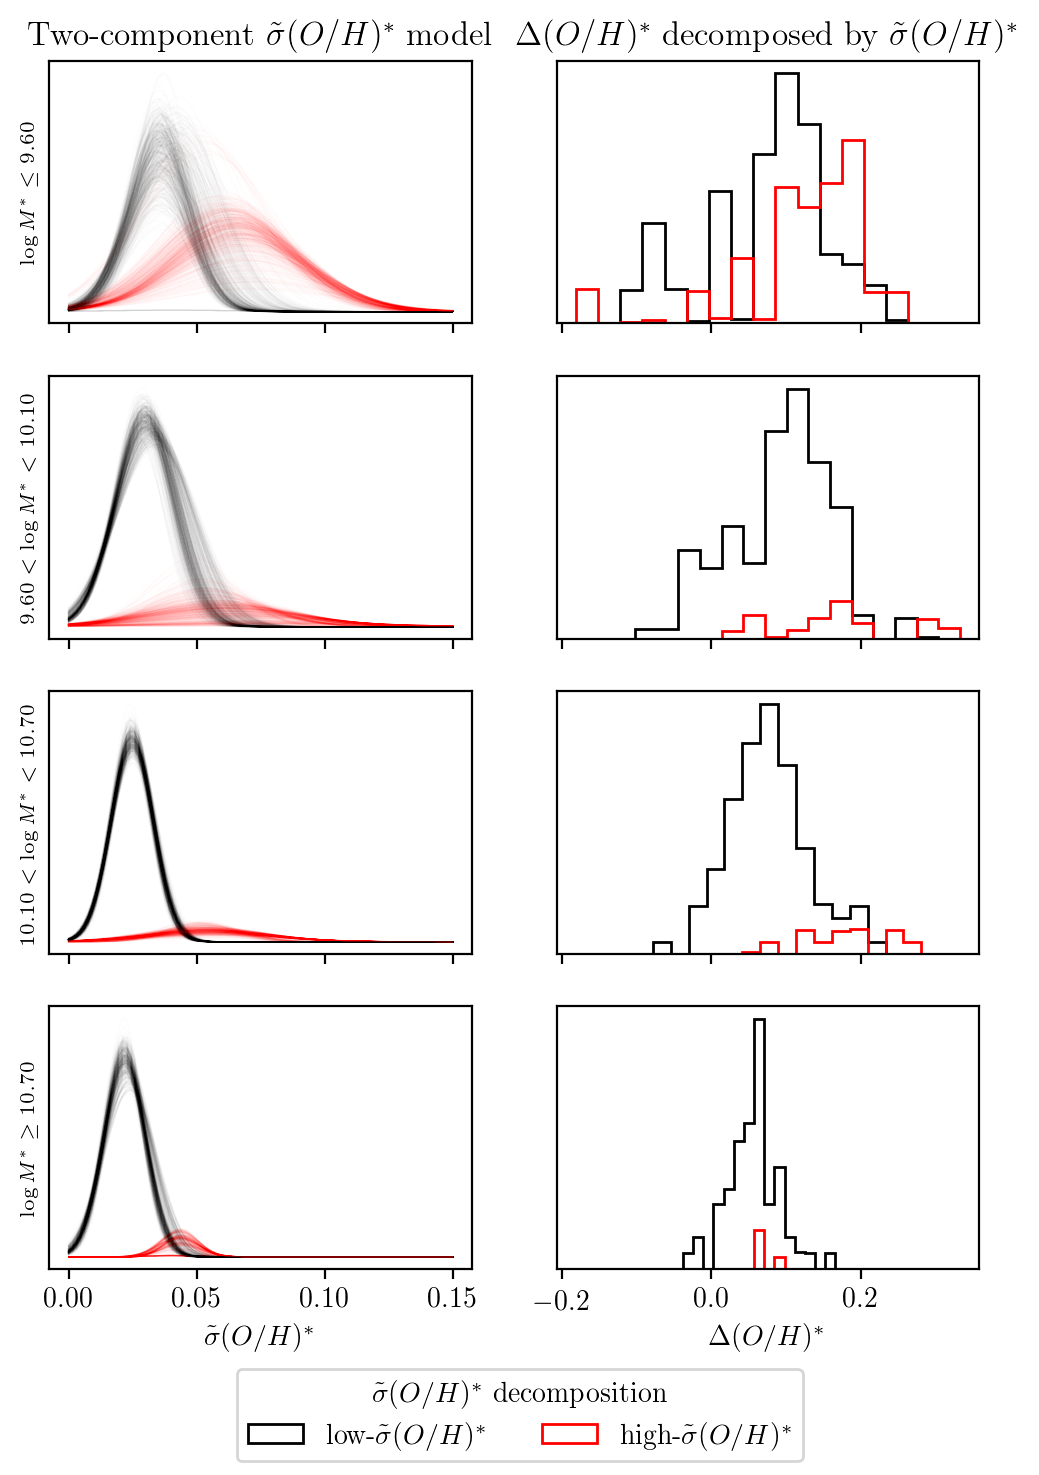
\includegraphics{sigma2comp_dec01_subplotmstar}
    \caption[Two-component decompositions of stellar mass bins' distributions by their scatter of their metallicity distribution at fixed radius.]{\fixspacing Decompositions of the $M^*$-separated sample of galaxies on the basis of their metallicity dispersion in the interval $1.25-1.75 ~ R_e$. All galaxies with well-measured decrements are used, regardless of HI observation or detection. Each row shows the decomposition results for one bin of total galaxy stellar mass. In the left-hand column are shown five-hundred two-component decompositions of \metdisp, under a bootstrap-resampling approach (80\% of points retained). The black (red) curves show the best-fit distributions of the low- (high-) -\metdisp populations. In the right-hand panel are shown the empirical distributions of \metdec for the low- and high-\metdisp populations (black and red), weighted by how often a galaxy is sorted into each population. Both populations appear to have relatively consistent modes across bins of stellar mass, though the low-\metdisp population is visually much more prominent at low stellar mass. Strikingly, the members of the high-\metdisp population tend to have high values of \metdec in the low- and intermediate-mass bins.}
    \label{fig:decomposition}
\end{figure*}

Within each stellar mass bin, the comparison (high-\metdisp) sample's median oxygen abundance in radial bin 1 ($\met_{comp,1}$) is taken as the observed, post-inflow metallicity ($\met_{obs}$). A range of possible pre-inflow metallicities ($\met_{in}$) are used, with the following limits
%
\begin{itemize}
    \item The median oxygen abundance in radial bin 1 of the fiducial sample ($\met_{fid,1}$)
    \item The average of $\met_{comp,1}$ and $\met_{fid,1}$
\end{itemize}
%

The metallicity of the accreted gas is set to one of two values obtained through a gas-regulator-model analysis of the same type as \citet{schaefer_19_accretion}, but using the \texttt{PG16-R2} metallicity calibrator: a value of 7.24 ($\sim 1/30 Z_{\odot}$) corresponds to the mean accreted metallicity of satellites of low-mass ($\logmstar < 10$) galaxies; and a value of 7.52 ($\sim 1/15 Z_{\odot}$) corresponds to the mean accreted metallicity of satellites of high-mass ($\logmstar > 10.5$) galaxies. While these metallicities by definition pertain to accretion by low-mass galaxies ($9 < \logmstar < 10$), and are therefore most appropriate to the two lowest-mass bins, they are realistic order-of-magnitude estimates. An alternative would be to adopt for higher-mass galaxies the typical metallicities of Milky Way high-velocity clouds (HVCs), which are somewhat sub-solar \citep{wakker_2004_hvc_bookchapter}, though not universally external in origin \citep{fox_2016_smithcloud}. We do not do show results for typical HVC metallicities, since the model is relatively insensitive to inflow metallicity.

$d_{in}$ is computed for each combination of $\met_{amb}$ and $\met_{in}$. The results are shown in Figure \ref{fig:oh-ambient_d-in_color-oh-obs}. We find that according to this picture of dilution by lower-metallicity gaseous inflows, local star-forming gas reservoirs encounter inflows with between 10\% and 90\% of ambient gas surface-density. The most massive, star-forming galaxies ($> 10^{10.7} {\rm M_{\odot}}$) seem to be somewhat distinct in that any inflow is constrained to be relatively small in magnitude compared with their existing local gas reservoirs; at high stellar mass, the multi-component decomposition of \metdisp does not heavily favor a high-\metdisp population, so this result is much less certain. In contrast, our simple model permits lower-mass galaxies to experience significant inflows ($10-100\%$) relative to their existing local gas reservoirs.

\begin{figure*}
    \centering
    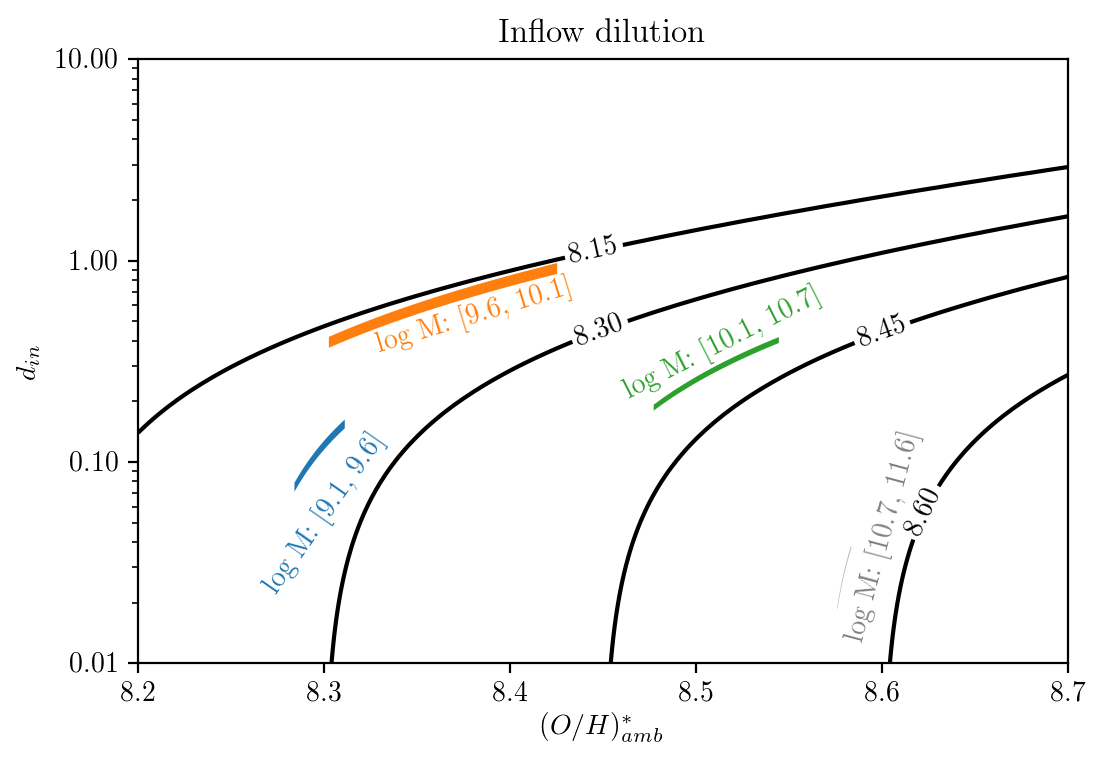
\includegraphics[width=\textwidth]{oh-ambient_d-in_color-oh-obs}
    \caption[A toy model of inflow's diluting effects on local metallicity and the mass increase of the associated gas reservoir.]{\fixspacing A toy model of inflow's effect locally on observed metallicity, assuming a range of ambient \& observed (pre-inflow \& post-inflow) metallicities, along with a range of inflow metallicities taken from a best-fit equilibrium model. A covariate range of local dilution factor and ambient metallicity (dependent on the choice of inflow metallicity) is shown for each of the four mass bins: the three lowest-mass bins are shown in color, since the two-component GMM used to estimate their pre- \& post-inflow metallicities is fairly well-characterized; the highest-mass bin is shown in gray, since the two-component decomposition is not reliable. Overlaid are contours representing the corresponding, average observed gas-phase metallicity for a given combination of $\met_{amb}$ and $d_{in}$.}
    \label{fig:oh-ambient_d-in_color-oh-obs}
\end{figure*}

The assumed ambient metallicity can be thought of as a reflection of how commonly inflows are incident at local scales upon a star-forming disk: if most regions are subject to more constant refueling (i.e. dilution), then the ambient metallicity is implied to be higher. That is, when only the most metal-rich tail of the metallicity distribution reflects the galaxy's recent star formation free from inflows, the local dilution must be stronger on average. This implies a large inflow covering fraction, so we evaluate the higher inflow dilution factors as somewhat less likely, given the large observed metallicity dispersion at fixed radius.

\subsection{Total \hi, dust, and extended UV disks in the accretion-dilution model}
\label{subsec:hifrac_diversity}

Under the toy model described above, in which the ambient ISM of galaxies is diluted by lower-metallicity gas with extragalactic origin, there should be a correspondence between the degrees of dilution and local H\textsc{i}-enhancement. In Section \ref{sec:modeling}, we computed that at total stellar masses of approximately $10^{9.6}-10^{10.1} M_{\odot}$ and accreted-gas metallicities of 7.24, local dilution factors are implied to be approximately 50\%, with a covering fraction somewhat less than one. Within individual stellar-mass bins, the higher-$\tilde{\sigma}(O/H)^*_1$ population has a larger HI mass fraction on average. This difference is most pronounced at intermediate mass: in the range $10^{9.6}-10^{10.1} M_{\odot}$, high-metallicity-dispersion galaxies have $\log \frac{M_{HI}}{M^*}$ enhanced by 0.25 dex, and for the range $10^{10.1}-10^{10.7} M_{\odot}$, the enhancement is 0.2 dex. Conversely, in the lower- and higher-mass bins, the enhancements are at most 0.1 dex.

To evaluate the possible inflow-induced enhancements in H\textsc{i} mass associated with the metallicity dilutions, we adopt a plausible, if simplistic description of a galaxy's H\textsc{i} radial mass profile: an exponential disk with an inner core (representing a transition to predominantly molecular gas) and an outer cutoff. Interior to an atomic-to-molecular transition radius $r_t$, the atomic gas mass surface density is constant; between $r_t$ and a cutoff radius $r_c$, the radial profile is an exponential, with a scale-length of $r_t$; and exterior to $r_c$, there is no gas. 

As an illustrative example, we consider the case of a hypothetical low-mass galaxy, with $M^* \sim 10^{9.85} {\rm M_{\odot}}$ and $\log \frac{M_{HI}}{M^*} \sim -0.2$ (the median of the low-\metdisp population for that stellar-mass bin). Following roughly a set of HI mass-size relations \citep[, as collated and expanded in \citealt{blue-bird_davis_2020}]{verheijen_sancisi_2001_hi-mass-size, wang_koribalski_2016_hi-mass-size, diskmass_x_martinsson_2016}, we estimate a physical HI disk cutoff radius of $\sim 20 {\rm kpc}$ (or roughly $8 R_e$). We rely on previous calibrations of bandpass-specific scale-lengths with respect to $r_{25}$ to estimate the dimensionless ratio $\frac{<h_{\Sigma_{tot~gas}} / r_{25}>}{<h_{0.7 \mu m} / r_{25}>} \approx 1.6$ \citep[see][Table 7]{casasola_2017_dustpedia-scalelengths}. In units of $R_e$, this ratio is adopted as $r_t$.

We will briefly use this model profile as a fiducial for a galaxy without an inflow, and evaluate possible inflow-related enhancements to it. Guided by our dilution model, we assume that a gaseous inflow provides a 50\% enhancement to local star-forming gas reservoirs, with a covering fraction of 50\%. Under this fiducial model, the mass fraction contained in the radial interval [$1.25 ~ R_e$, $1.75 ~ R_e$] is approximately 6\%. Consequently, an inflow with the characteristics described above would affect a minuscule ($\sim 1\%$, or $< 0.01 ~ {\rm dex}$) enhancement in the \emph{global} gas mass. This admittedly-limiting case is substantially less than typical differences between HI fractions in low- and high-\metdisp populations (0.05 - 0.25 dex). In contrast, an inflow affecting all radii between $1.25 R_e$ and $r_c$ would enhance a galaxy's global HI mass by $\sim 0.1 ~ {\rm dex}$ (assuming the same covering fraction and local gas enhancement). This is more plausible, but still less than the 0.25 dex the population comparison suggests. As the assumed outer extent of the inflow grows to exceed $r_c$, the enhancement in total gas mass becomes insensitive to $r_c$; in order to reach the large HI fractions of the high-\metdisp population, the inflow's radial profile must become shallower (i.e., the scale-length must increase). For example, an inflow profile incident only on $r > 1.25 ~ R_e$, with a 50\% local mass enhancement at $1.25 ~ R_e$, $r_t = 2 ~ R_e$ (a shallower slope than the fiducial), and $r_c = 16 ~ R_e$ (a larger cutoff radius than the fiducial) achieves a global gas mass enhancement of nearly $0.2 ~ {\rm dex}$. Modulating the inflow covering fraction with respect to radius is qualitatively similar to adopting a longer inflow scale-length: if this were the case, metallicity profiles would steepen when measured at larger radius, but \metdisp would lessen (as the metallicity distribution function at fixed radius becomes unimodal). These examples illustrate that if an inflow is responsible for the abundance trends found in this work, there ought to be a \emph{significant} gaseous component at large galactocentric radius.

An extended gaseous tail could also form stars, albeit with lower efficiency \citep{rafelski_2016}. Indeed, a star-forming ``plume" has been reported around M101 \citep{mihos_2013_m101-uvdisk}, as well as associated with MaNGA ALM-region candidates \citep{hwang_2019_manga_almrs}. That said, no statistical enhancement of NUV-to-$r$-band Petrosian radius ratio (which might signal low-efficiency star formation in the inflowing gas) is found in high-\metdisp galaxies compared to peer galaxies at similar mass.

Inflows, if present, may also have a dust component, since their metallicity is strongly constrained to be nonzero. So, for an inflow with large enough mass and dust-to-gas ratio, the stellar populations may appear to have a greater attenuating dust foreground with respect to the typical galaxy without an inflow. To investigate this possibility, we adopt the importance-sampling inference method of \citet{pace_19a_pca}, and use a representative library of 40,000 synthetic ``training" SFHs and their spectra to infer the foreground V-band optical depth arising from a two-component dust model \citep{charlot_fall_00}. However, we find that in the radial interval $1.25-1.75 ~ R_e$, the inferred V-band optical depth (arising from both the diffuse and dense dust components) is not noticeably enhanced in galaxies inferred to belong to the high-\metdisp population, at fixed stellar mass. This lack of visible foreground dust enhancement could be explained by a few factors: first, the number of high-\metdisp galaxies in each mass bin is small by construction. Second, the geometry of the inflow with respect to the line of sight is unknown, and an inflow may not produce an attenuation signature along all lines of sight. Finally, at the expected inflow metallicities, the dust-to-gas ratio is likely a factor of several smaller than at ambient metallicities \citep{kahre_walterbos_2018_legus_dusttogas}. Thus, the local dilution observed may not produce a detectable signature at all.


